\chapter{Introduction}

\section{Background}\label{sec:i-background}

\subsection{High Performance Computing}

% HPCとはなにか
Recent advancement in science has significantly benefited from High
Performance Computing~(HPC). Scientists are able to simulate nature on HPC
systems. HPC helps scientists to develop a better understanding of nature and
answer fundamental questions about our surrounding environment by executing
high-resolution computational models of natural phenomena.

% HPCの応用分野
A wide spectrum of science has taken advantage of the massive computing
capability provided by HPC\@. Various phenomena ranging from atomic scale to
cosmological scale intractable to experimentally observe or reproduce are
simulated on HPC systems. For instance, molecular dynamics simulation reveals
the molecular-level structure and property of matter and their interaction.
This knowledge is used to design better drugs and materials. Earthquake and
Tsunami simulation allows us to predict the impact of seismic activities and
prepare for natural disasters. In addition to simulation applications, data
analysis and machine learning applications are also starting to leverage HPC
systems.

% HPCシステムの計算性能の推移
Scientists are trying to tackle increasingly larger and more complex problems.
This continuous demand from domain scientists has kept pushing the performance
HPC systems forward. Figure~\ref{fig:top500-rmax} shows the development of
computing performance of HPC systems based on the data published by the
Top500~\autocite{top500} list. The Top500 list is a biannual list of 500 most
powerful HPC systems measured by the maximal LINPACK benchmark performance
achieved. The plot clearly indicates the exponential increase in performance
over the past 20 years. Researchers and engineers are striving to sustain this
exponential growth in performance and exascale~(Exa FLOPS) in the near future.
To achieve this daunting technological challenge, every aspect of the HPC
system including hardware, operating system, middleware and application need
to be greatly improved, optimized and even redesigned.

\begin{figure}
    \centering
    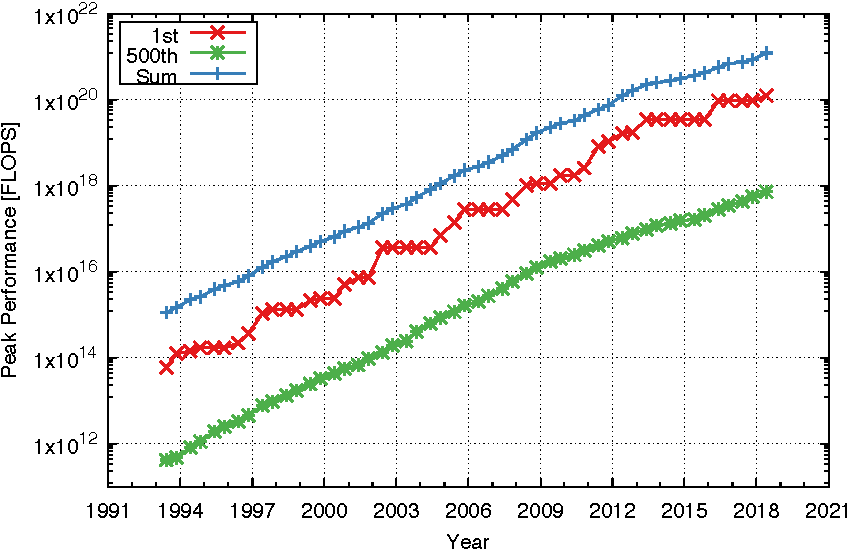
\includegraphics{top500_rmax}
    \caption{Performance Development of Top500 HPC Systems~\autocite{top500}}%
    \label{fig:top500-rmax}
\end{figure}

\subsection{Cluster Architecture}

% クラスタとはなにか
Modern HPC systems mostly adopt \emph{cluster} architecture to achieve their
massive computing performance. In fact, 87\% of the recent Top500 systems
(July 2018) are based on cluster architecture. A cluster is an aggregation of
interconnected computers working cooperatively. Computers that constitute a
cluster perform computation in parallel and exchange data with each other to
required for the computation.

% クラスタの構成要素
Figure~\ref{fig:cluster} shows the architectural overview of a typical
cluster. A cluster consists of multiple computers~(\emph{i.e.,\ computing
nodes}) and a high-performance network that integrates~(\emph{i.e.,\
interconnect}) them together as a single system. Since many users share a
single cluster, a \emph{job scheduler} is deployed to effectively manage the
computing resources in a cluster. A job scheduler accepts jobs from users and
determines when to run each job. The scheduler is also responsible for
allocating computing nodes to a job and launching jobs on allocated nodes.
Furthermore, a shared file systems is usually deployed to store the input and
output data of applications executed on the cluster.

\begin{figure}
    \centering
    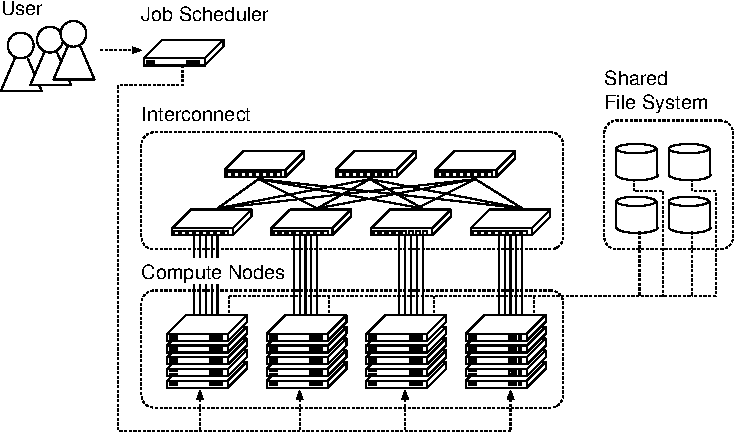
\includegraphics{cluster}
    \caption{Cluster Architecture}%
    \label{fig:cluster}
\end{figure}

% クラスタの規模拡大
There has been an increasing trend in the number of computing nodes that
compose a cluster. Although the computing performance of a single processor
and computing node have been steadily improving, the growth is not fast enough
to meet the high demand for computing power from the users. Therefore, the
designers of HPC systems need to increase the number of computing nodes to
further improve the total computing performance of the cluster. As a result, a
single cluster accommodates up to tens of thousands of computing nodes and
millions of cores nowadays.

% 相互結合網の重要性
The performance of communication between computing nodes over the interconnect
is essential to the scalability of the cluster. In general, computing nodes
need to frequently communicate with each other during the parallel computation
to exchange intermediate results. If the communication between computing nodes
becomes a bottleneck, simply adding more nodes to the cluster does not
increase the total performance of the cluster. Therefore, great effort has
been put to the research and development of high-performance interconnects.

\subsection{Interconnect}\label{sec:i-interconnect}

There are mainly two design goals of a high-performance interconnect: high
bandwidth and low latency.

% 通信規格
Ethernet~\autocite{Trowbridge2007} and InfiniBand~\autocite{Buyya2009} are
network technology standards commonly utilized for interconnects. Ethernet is
a long-standing network technology that has been ubiquitously used in both
local area networks and wide are networks. InfiniBand, on the other hand, is a
network standard specifically designed with HPC in mind. InfiniBand offloads
most of its protocol stack onto hardware and realizes mechanisms such as
kernel bypassing and Remote Direct Memory Access~(RDMA) to reduces the
communication latency. In addition to Ethernet and InfiniBand, some HPC system
vendors develop proprietary interconnects for their systems. In this
dissertation, we assume that Ethernet is being used for the interconnect.

% トポロジ
Topology is a key factor that determines the performance of an interconnect.
A fully-connected topology is ideal since it has dedicated links between any
pair of computing nodes. However, implementing a fully-connected topology in a
large scale cluster is unrealistic due to extremely high cost and complexity.
Therefore, various topologies have been proposed that take the balance
between cost and performance. Figure~\ref{fig:topology} illustrates some of
the popular topologies. For example, fat-tree~\autocite{Leiserson1985},
multi-dimensional torus~\autocite{Adiga2005,Ajima2012},
dragonfly~\autocite{Kim2008}, and hypercube~\autocite{Dally2003} have been
widely adopted as interconnect topologies in HPC systems.

\begin{figure}
    \centering
    \begin{subfigure}{.45\linewidth}
        \centering
        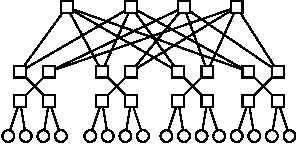
\includegraphics[scale=1.2]{topology-fattree}
        \caption{Fat-tree}%
        \label{fig:topology-fattree}
    \end{subfigure}
    \begin{subfigure}{.45\linewidth}
        \centering
        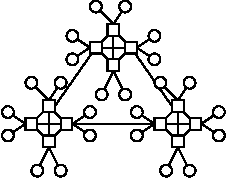
\includegraphics[scale=1.2]{topology-dragonfly}
        \caption{Dragonfly}%
        \label{fig:topology-dragonfly}
    \end{subfigure}
    \par\bigskip
    \begin{subfigure}{.45\linewidth}
        \centering
        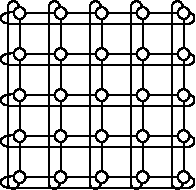
\includegraphics[scale=1.2]{topology-torus}
        \caption{2D Torus}%
        \label{fig:topology-torus}
    \end{subfigure}
    \begin{subfigure}{.45\linewidth}
        \centering
        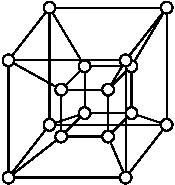
\includegraphics[scale=1.2]{topology-hypercube}
        \caption{4D Hypercube}%
        \label{fig:topology-hypercube}
    \end{subfigure}
    \caption{Topology of Interconnects}%
    \label{fig:topology}
\end{figure}


Mostly, the interconnects of computer cluster systems are full-bisection.
The bisection bandwidth for an interconnect is defined as the minimum
bandwidth between two counterparts of the interconnect. A full-bisection
interconnect is an interconnect whose bisection bandwidth is larger or equal
to the aggregated bandwidth between computing nodes. Interconnects that are
not full-bisection are referred as oversubscribed. Full-bisection interconnect
design are preferred since such interconnect does not suffer from network
contention even in the worst case scenario where all computing nodes
communicate with each other at maximum speed of their network interfaces. This
characteristic is beneficial for application since it removes the need to be
aware of the current contention state of the interconnect. However, there is a
common problem with full-bisection design: the financial cost to implement
such a design increases superlinearly as the number of node scales out.
% OversubscriptionとTapered fat-treeについて触れる

\subsection{Message Passing Interface}\label{sec:i-mpi}

% MPIとは
Message Passing Interface (MPI)~\autocite{MPIForum2012} is a \emph{de
facto} standard specification for inter-process communication libraries
used to develop parallel applications running on distributed memory system
such as clusters. MPI defines a suite of communication primitives that helps
application developers to build parallel distributed applications that require
complex communications among computing nodes.

% 相互結合網の抽象化
A remarkable feature of MPI is that it abstracts the underlying network
of clusters. As shown in Fig.~\ref{fig:mpi-arch}, each interconnect technology
requires the developers to use a different set of APIs. MPI hides the this
incoherence and allows developers to build applications without forcing them
to study the detailed architecture or structure of the underlying network. For
instance, every process is identified by a \emph{rank} number, a consecutive
non-negative integer. The mapping between rank numbers and network addresses
is automatically handled by the MPI library. Communication can be restricted
into a particular group of processes, which is called a \emph{communicator}.
These abstractions make MPI applications portable and easy to be ported to
different computer clusters.

\begin{figure}
    \centering
    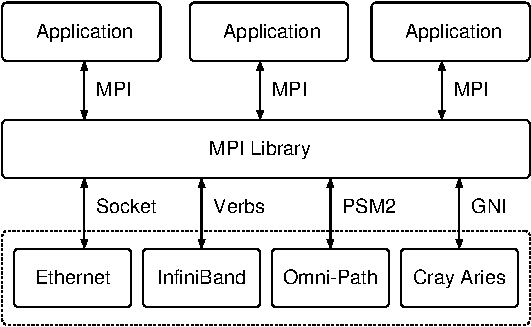
\includegraphics{mpi-arch}
    \caption{Abstraction Provided by MPI}%
    \label{fig:mpi-arch}
\end{figure}

% 1対1通信と集団通信
The communication primitives defined in MPI can be roughly categorized into
point-to-point communication and collective communication. Point-to-point
communication is a communication between one sender and one receiver. On the
other hand, collective communication involves a group of processes. These
communication primitives help application developers to implement complex
parallel algorithms. Table~\ref{tbl:mpi-primitives} shows some representative
examples of MPI primitives.

\begin{table}
    \centering
    \caption{Examples of MPI primitives}%
    \label{tbl:mpi-primitives}
    \begin{tabular}{lll}
        \toprule
        Name & Category & Description \\ \midrule
        MPI\_Send/MPI\_Recv & Point-to-point & Blocking send/receive \\
        MPI\_Isend/MPI\_Irecv & Point-to-point & Non-blocking send/receive \\
        MPI\_Bcast & Collective & Broadcast \\
        MPI\_Reduce & Collective & Reduction \\
        MPI\_Allreduce & Collective & Broadcast result of reduction \\
        MPI\_Gather & Collective & \begin{tabular}[c]{@{}l@{}}Aggregate pieces of data from\\ processes into a single process\end{tabular} \\
        MPI\_Alltoall & Collective & \begin{tabular}[c]{@{}l@{}}Perform MPI\_Gather from all\\ processes\end{tabular} \\
        \midrule
    \end{tabular}
\end{table}

% MPIの高速化
Until today, countless scientific applications have been developed by
utilizing MPI\@. Accompanied by the recent scale-out of clusters, the
execution time of MPI primitives has become a critical factor that determines
the total performance of these applications using MPI\@. In other words, the
total performance of MPI applications can be improved by optimizing the
performance of MPI communications. For this reason, researchers have been
striving to improve the communication performance of MPI from various aspects.

\subsection{Problem and Motivation}

% アプリケーションの通信パターン
The inter-process communication of MPI applications shows a distinctive
pattern. This pattern varies depending on the application and originates from
the mathematical model, numerical algorithm, and parallelization strategy.
Figure~\ref{fig:stencil3d} shows the communication pattern of a
three-dimensional finite-difference solver that performs nearest neighbor
communication as an example. In this figure, the total size of messages sent from
a process to another process is visualized using a heat map. The visual
representation evidently exhibits a regular and local pattern along the
diagonal that originates from the nearest neighbor communication required by
the finite-difference method.
% 論文中の通信パターンの定義をここで書く?

\begin{figure}
    \centering
    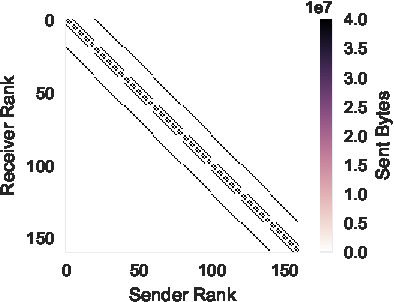
\includegraphics[width=0.6\linewidth]{stencil3d}
    \caption{Communication Pattern of an Application}%
    \label{fig:stencil3d}
\end{figure}

% 相互結合網は通信パターンを無視している
The design of an interconnect could be highly optimized for an
application by taking the communication pattern of applications into account.
For instance, an interconnect with a three-dimensional torus topology would be
ideal for an application that performs nearest neighbor communication in 3D
space. However, this approach is infeasible when designing a real-world
cluster. This is because HPC systems are shared by many users, where each user
runs various applications on the cluster. Furthermore, Therefore, in contrast
to the application-dependent communication pattern, the interconnect is
inherently application-agnostic.

% 問題
As a result, under a certain combination of communication pattern and
interconnect, an imbalance of the packet flow in the interconnect can occur.
The imbalance can lead to the concentration of traffic on a link in the
interconnect and slow down of MPI communication that uses the link. The
degraded MPI communication can ultimately lead to a serious degradation of
total application performance.

% 関連研究
A  number of previous studies have tried to address the mismatch between
application application-dependent communication patterns and
application-agnostic interconnects. A class of approaches tries to adapt
the communication pattern of applications to the interconnect.
For instance, interconnect-aware MPI
collectives~\autocite{Kumar2016,Kumar2014,Gong2015,Adachi2013} have been
developed to improve the performance of MPI collectives by taking into account
the interconnect of a cluster. MPI implementation often leverage tree-based
algorithms to aggregate or distribute messages from or to processes.
Interconnect-aware MPI collectives use the information on the interconnect to
build a delivery tree that matches the underlying interconnect of the cluster.
Another class of approaches tries to optimize the placement of MPI processes
on the computing nodes~\autocite{Michelogiannakis2017,Hoefler2011,Choi2017}.
In this approach, the communication pattern of an application is considered as
a weighted graph where nodes represent processes and edges represent the
volume of data exchanges between two processes. Various heuristic algorithms
are proposed to embed the communication pattern graph graph onto the
interconnect topology.

% 相互結合網の動的制御は未だ研究が進んでいない
To this date, however, there has been little studies on adapting the
interconnect to the communication pattern of applications. This is mostly
because it has been assumed that flexibly and dynamically reconfiguring the
interconnect at runtime is infeasible. However, this assumption might not hold
anymore with the recent emergence of programmable networking architecture that
allows reconfiguring the interconnect on-the-fly.

\subsection{Software-Defined Networking}

% SDN
Software-Defined Networking (SDN) is a novel networking architecture
that separates the control plane and data plane into different devices.
In conventional networking architectures, the decision on how to handle
packets (control plane) and the packet transfer (data plane) are
implemented as unified and inseparable features. The separation of the
control plane and data plane has allowed SDN to deliver the following
three benefits:

\begin{itemize}
\item
  \emph{Programmable}: The control plane can be handled by a software
  controller. Network operators can program controllers tailored for
  their needs.
\item
  \emph{Dynamic}: SDN allows the controller to quickly reconfigure the
  network. For instance, it is possible to dynamically optimize packet
  flow in the network based on the real-time traffic pattern.
\item
  \emph{Centralized}: A centralized controller configures the entire
  SDN-enabled network, thus reducing efforts to administer and manage
  the network. In conventional networking architectures, the operators
  need to configure each network device separately because the control
  plane is distributed on individual devices.
\end{itemize}

\begin{figure}
    \centering
    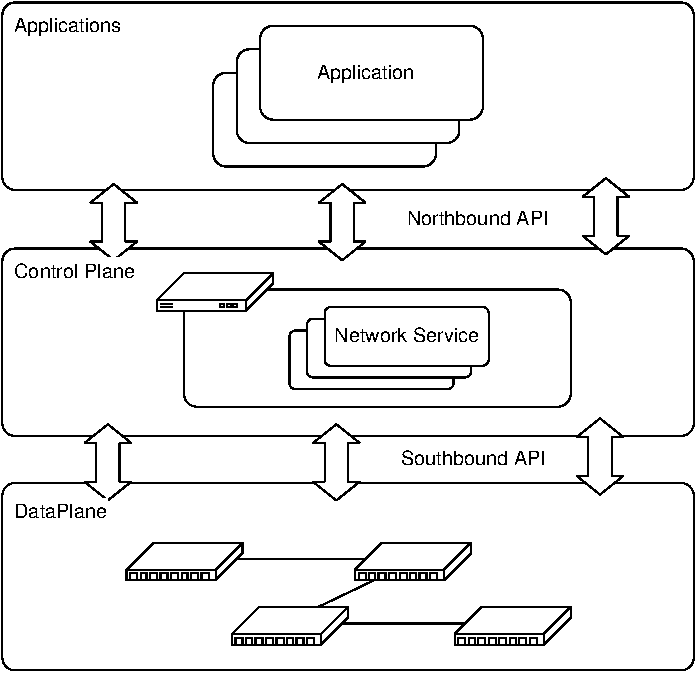
\includegraphics{sdn}
    \caption{Software-Defined Networking Architecture}%
    \label{fig:sdn-architecture}
\end{figure}

% OpenFlow
\emph{OpenFlow}~\autocite{McKeown2008} is a widely accepted open
standard of SDN\@. In an OpenFlow-enabled network, the data plane is
handled by OpenFlow switches. Every OpenFlow switch holds a logical
construct called \emph{flow table}, which is a collection of \emph{flow
entries}. Each flow entry defines what kind of packet control should be
performed on what kind of packets (Fig.~\ref{tbl:flow-table}). Every
time a packet arrives at an OpenFlow switch, the switch looks up a
matching flow entry in its flow table using the header fields of the
packet. Once a matching flow entry is found, the action of the matched
flow entry is applied to the packet.

The OpenFlow controller is responsible for the control plane. It manages
the flow table of switches by adding, removing and modifying flow
entries. The controller and switches communicate with each other by
asynchronously exchanging messages defined in the OpenFlow protocol. One
of the frequently used messages is the \emph{packet-in} message, which
is sent out from a switch to the controller when no matching flow entry
is found for an incoming packet. In response, the controller can send a
\emph{modify flow entry} message to install a new flow entry on the
switch.

\begin{figure}
    \centering
    \begin{tabular}{lllll}
        \toprule
        \multicolumn{3}{c}{Header Fields}            &  Action                  \\ \midrule
        Dst MAC           & Src IP     & Dst IP      &                          \\ \midrule
                          & 192.0.2.12 & 192.0.2.34  & Output to port 1         \\
                          & 192.0.2.34 & 192.0.2.56  & Output to port 2         \\
        ff:ff:ff:ff:ff:ff &            &             & Output to port 1 and 2   \\
        72:42:c1:e4:75:8c &            &             & Drop                     \\
        \bottomrule
    \end{tabular}
    \caption{An example of a flow table}%
    \label{tbl:flow-table}
\end{figure}

% もう一枚図を追加?

\section{Research Objective}

As discussed in Section~\ref{sec:i-background}, the mismatch between
application-dependent communication patterns and application-agnostic
interconnects have lead to the imbalance of packet flow in the interconnect.
This dissertation aims to address this problem by establishing a programmable
interconnect control that dynamically controls the packet flow in the
interconnect based on the communication pattern of applications.

\begin{figure}
    \centering
    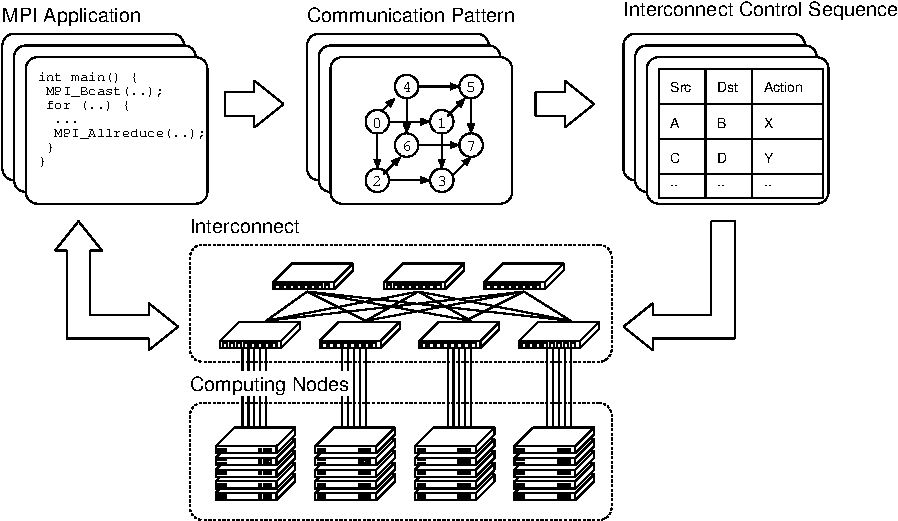
\includegraphics{objective}
    \caption{Envisioned Interconnect Control}%
    \label{fig:objective}
\end{figure}

Figure~\ref{fig:objective} illustrates the envisioned interconnect control
architecture. The overall idea of this architecture is as follows. First, the
communication pattern of MPI communication is extracted from the application.
Then, a sequence of interconnect control instructions is generated based on
the communication pattern. Finally, the interconnect control sequence is
applied to the interconnect using programmable interconnect technology.
There are three central challenges in realizing such programmable interconnect:

\begin{enumerate}
\item \emph{Analyzing the Packet Flow in the Interconnect}:
    To effectively control the packet flow in the interconnect, we first need
    to analyze and understand the packet flow generated in the interconnect
    when running an application on the cluster.
\item \emph{Accelerating MPI Communication by Dynamic Control of Interconnect}:
    Given a communication pattern of an application and an interconnect,
    we need to determine how to control the packet flow in the interconnect to
    mitigate imbalance and improve the performance of MPI communication.
\item \emph{Coordinating the Execution of Application and Interconnect Control}:
    The communication pattern of the application changes with the execution of
    the application. Therefore, the interconnect control must be performed in
    accordance with the execution of application.
\end{enumerate}

\section{Organization of the Dissertation}

The rest of this dissertation is organized as follows:

% アプリケーションが相互結合網内に生成するパケット
フローの解析手段を実現
In Chapter~\ref{sec:ii}, we propose PFAnalyzer, a toolset for analyzing packet
flow in interconnects to address the first challenge. Interconnect simulators
come in handy especially when investigating the performance characteristics of
interconnects with different topologies and parameters. However, little effort
has been put towards the simulation of packet flow in dynamically controlled
interconnects, while simulators for static interconnects have been extensively
researched and developed. To facilitate analysis on the performance
characteristics of dynamic interconnects, we have developed PFAnalyzer.
PFAnalyzer is a pair of two tools: PFSim, an interconnect simulator
specialized for dynamic interconnects, and PFProf, a profiler. PFSim allows
interconnect researchers and designers to investigate congestion in the
interconnect for an arbitrary cluster configuration and a set of communication
patterns collected by PFProf. PFAnalyzer is used to demonstrate how
dynamically controlling the interconnects can reduce congestion and
potentially improve the performance of applications.

% MPI集団通信を高速化するパケットフロー制御アルゴリズムを配備可能なフレームワークを構築
In Chapter~\ref{sec:iii}, we address the second challenge by proposing a
framework that accelerates MPI collectives by controlling the packet flow in
the interconnect. We integrate the network programmability provided by
Software-Defined Networking into MPI collectives so that collectives are able
to effectively utilize the bandwidth of the interconnect. In particular, we
aim to reduce the execution time of MPI\_Allreduce, a frequently used MPI
collective communication in many simulation codes. An experiment conducted on
a cluster system with fat-tree interconnect indicates that our proposed
MPI\_Allreduce is superior to MPI\_Allreduce in Open MPI implementations.

% 通信と計算が連係動作する新たなクラスタアーキテクチャを確立
In Chapter~\ref{sec:iv}, the third challenge is addressed. This chapter
proposes UnisonFlow, a software-defined coordination mechanism that performs
network control in synchronization with the execution of applications. An
experiment conducted on a real computer cluster verifies that the interconnect
control can be successfully performed in synchronization with the execution of
the application. Furthermore, the synchronization is performed with a low
overhead and its performance penalty is practically negligible.

Chapter~\ref{sec:v} concludes this dissertation and describes the future work.
